\documentclass[10pt,a4paper]{article}

\usepackage[T1]{fontenc}
\usepackage[utf8]{inputenc}
\usepackage{lmodern}
\usepackage[margin=2.3cm]{geometry}
\usepackage{amsmath,amssymb}
\usepackage{graphicx}
\usepackage{booktabs}
\usepackage{longtable}
\usepackage{array}
\usepackage{url}
\usepackage{xcolor}
\usepackage{microtype}
\usepackage[hidelinks]{hyperref}
\usepackage{orcidlink}
\usepackage{caption}
\captionsetup{font=small,labelfont=bf}
\setlength{\parskip}{0.4em}
\setlength{\parindent}{0pt}

\graphicspath{{../figures/}}
% Generated by data/extract.py from the committed files. Do not edit.
\newcommand{\productVersion}{0.02.000}
\newcommand{\nClassical}{10}
\newcommand{\nSota}{9}
\newcommand{\nBeyond}{5}
\newcommand{\nLadder}{24}
\newcommand{\nCases}{14}
\newcommand{\nCasesBaked}{13}
\newcommand{\nMethodsBaked}{24}
\newcommand{\nMethodCells}{111}
\newcommand{\minTraps}{9}
\newcommand{\maxTraps}{1024}
\newcommand{\nDisordered}{819}
\newcommand{\atomLambda}{850}
\newcommand{\atomFocal}{6}
\newcommand{\atomNa}{0.5}
\newcommand{\atomNimm}{1}
\newcommand{\atomNpix}{256}
\newcommand{\atomPitch}{20}
\newcommand{\atomPad}{2}
\newcommand{\atomBin}{0.498}
\newcommand{\atomHalf}{127.5}
\newcommand{\beadLambda}{1064}
\newcommand{\beadFocal}{2.4}
\newcommand{\beadNa}{1.2}
\newcommand{\beadNimm}{1.33}
\newcommand{\beadNpix}{256}
\newcommand{\beadPitch}{10}
\newcommand{\beadPad}{2}
\newcommand{\beadBin}{0.499}
\newcommand{\beadHalf}{127.7}
\newcommand{\devcLambda}{850}
\newcommand{\devcFocal}{3}
\newcommand{\devcNa}{0.5}
\newcommand{\devcNimm}{1}
\newcommand{\devcNpix}{128}
\newcommand{\devcPitch}{20}
\newcommand{\devcPad}{2}
\newcommand{\devcBin}{0.498}
\newcommand{\devcHalf}{63.8}
\newcommand{\voluLambda}{850}
\newcommand{\voluFocal}{2.56}
\newcommand{\voluNa}{0.5}
\newcommand{\voluNimm}{1}
\newcommand{\voluNpix}{128}
\newcommand{\voluPitch}{20}
\newcommand{\voluPad}{1}
\newcommand{\voluBin}{0.850}
\newcommand{\voluHalf}{54.4}
\newcommand{\devcBits}{4}
\newcommand{\devcFill}{0.85}
\newcommand{\devcFlicker}{0.05}
\newcommand{\notBakedSentence}{every one of them ran in at least one case}
\newcommand{\liveTests}{92}
\newcommand{\liveGpuS}{0.31 to 0.32}
\newcommand{\liveCpuS}{1.5 to 1.6}
\newcommand{\liveAdapter}{an integrated Intel gen-12lp adapter}
\newcommand{\liveIterMs}{24}
\newcommand{\liveBudgetMs}{1500}
\newcommand{\liveTraceKiB}{256}
\newcommand{\liveFixtures}{46}
\newcommand{\liveTol}{10^{-9}}
\newcommand{\accFourFlatEff}{0.939}
\newcommand{\accFourFlatUni}{0.604}
\newcommand{\accBFourRatio}{1.57}
\newcommand{\accBFourEffDrop}{1.9}
\newcommand{\accBFourPointing}{1.04}
\newcommand{\accBFiveHv}{0.8190}
\newcommand{\accBFiveHvBase}{0.8018}
\newcommand{\accBFiveDomFour}{7}
\newcommand{\accBFiveDomFive}{8}
\newcommand{\benchTimes}{0.05, 1, 60}
\newcommand{\bakeCeightMsevenSigma}{13.4}
\newcommand{\bakeCeightBOneSigma}{7.1}
\newcommand{\bakeCeightRatio}{1.9}
\newcommand{\bakeCeightEffRatio}{0.966}
\newcommand{\execAtoms}{6,100}
\newcommand{\execSpread}{11.4}
\newcommand{\benchSeeds}{20}
\newcommand{\benchGrids}{128, 256, 512}
\newcommand{\benchIters}{10, 30, 100}
\newcommand{\benchGeometries}{7}
\newcommand{\benchRows}{63}
\newcommand{\benchSkipped}{62}
\newcommand{\benchMethodsMeasured}{M01}
\newcommand{\benchNMeasured}{1}
\newcommand{\benchNProtocol}{24}
\newcommand{\fbCOneStart}{9.1}
\newcommand{\fbCOneEnd}{0.02}
\newcommand{\fbCOneSteps}{5}
\newcommand{\fbCTwoStart}{20.1}
\newcommand{\fbCTwoEnd}{1.34}
\newcommand{\fbCTwoSteps}{20}
\newcommand{\fbCThreeStart}{22.3}
\newcommand{\fbCThreeEnd}{1.44}
\newcommand{\fbCThreeSteps}{3}
\newcommand{\fbCThirteenStart}{22.0}
\newcommand{\fbCThirteenEnd}{0.44}
\newcommand{\fbCThirteenSteps}{5}
\newcommand{\beadFc}{70.0}
\newcommand{\beadKappa}{4.01}
\newcommand{\atomFc}{107200}
\newcommand{\atomOmega}{109092}
\newcommand{\cghN}{162}
\newcommand{\cghMed}{1.140}
\newcommand{\cghQOne}{1.102}
\newcommand{\cghQThree}{1.160}
\newcommand{\cghNetMs}{35}
\newcommand{\cghBudgetS}{7.35}
\newcommand{\cghAcHybrid}{0.687}
\newcommand{\cghAcMnine}{0.600}
\newcommand{\cghBytes}{4.67}
\newcommand{\cghSteps}{16000}
\newcommand{\cghParity}{8.4\times 10^{-6}}
\newcommand{\cghLatticeRatio}{1.162}
\newcommand{\cghRingRatio}{1.100}
\newcommand{\cghRandomRatio}{1.147}
\newcommand{\cghMixedRatio}{1.118}
\newcommand{\cghGfiveRatio}{1.065}
\newcommand{\cghPlaneRatio}{1.188}
\newcommand{\cghShareAbove}{100}
\newcommand{\cghTwoDMed}{0.9994}
\newcommand{\cghTwoDN}{219}
\newcommand{\wsModelIt}{8}
\newcommand{\wsRandomIt}{14}
\newcommand{\wsRatio}{1.75}
\newcommand{\wsControlIt}{9}
\newcommand{\wsControlNever}{40}
\newcommand{\wsModelNever}{47}
\newcommand{\wsEffDiff}{4.2}
\newcommand{\wsN}{66}
\newcommand{\wsNfixModel}{3}
\newcommand{\wsNfixRandom}{12}
\newcommand{\nBothFourSeven}{9}
\newcommand{\medSigmaMfour}{18.7}
\newcommand{\medSigmaMseven}{0.01}
\newcommand{\minEffMseven}{0.453}
\newcommand{\maxEffMseven}{0.817}
\newcommand{\nContracts}{11}
\newcommand{\nContractsAvailable}{7}


% Page-1 header block (conventions/manuscript-header-standard.md). The four document macros are set by the
% publishing tool when the version DOI is reserved.
\newcommand{\doctype}{Technical report}
\newcommand{\docversion}{v0.02.000}
\newcommand{\docdate}{29 October 2026}
\newcommand{\versiondoi}{10.5281/zenodo.NNNNNNNN}
\newcommand{\conceptdoi}{10.5281/zenodo.NNNNNNNN}
\newcommand{\docrepo}{github.com/fsantibanezleal/CEFOP\_DinHot}
\newcommand{\headerblock}{%
\begin{center}
\fbox{\parbox{0.94\textwidth}{\small\raggedright
\textbf{\doctype} \quad$\cdot$\quad \docversion, \docdate \quad$\cdot$\quad Licence CC BY 4.0\\[2pt]
CAOS open-research programme \quad$\cdot$\quad CEFOP\_DinHot, holographic optical trap studio\\[2pt]
Version DOI \href{https://doi.org/\versiondoi}{\texttt{\versiondoi}} \quad$\cdot$\quad
concept DOI (always latest) \href{https://doi.org/\conceptdoi}{\texttt{\conceptdoi}}\\[2pt]
Not peer reviewed. Source code, data and computational records: \href{https://\docrepo}{\texttt{\docrepo}}
}}
\end{center}
\vspace{4pt}}

\begin{document}

\title{DinHot: A Holographic Optical Trap Studio Comparing Classical, State-of-the-Art\\ and Beyond-State-of-the-Art Hologram Methods on a Device Model}
\author{Felipe Santib\'a\~nez-Leal~\orcidlink{0000-0002-0150-3246}\\
\small CAOS open-research programme, Santiago, Chile\\
\small \texttt{fsantibanez@gmail.com}}
\date{}
\maketitle
\vspace{-1.2em}
\headerblock

\begin{abstract}
A phase-only spatial light modulator in the pupil of a microscope objective can form hundreds to thousands of optical
traps at once, but only if the phase pattern it displays is computed well: the pattern fixes how much light reaches the
traps, how equal the traps are, where stray light goes, how the pattern survives a real device, and how fast it can be
recomputed when traps move. DinHot is an open studio that runs \nLadder{} ladder methods (\nClassical{} classical,
\nSota{} state of the art, \nBeyond{} beyond it) on the same task, with the same seeds, metrics and device model, in
Python as the reference and in a TypeScript port that runs live in a browser. We describe the optical and device model,
the methods with the measured acceptance of each, \nCases{} cases from a $3\times3$ array to a disordered
\nDisordered-trap array and shaped potentials, the benchmark protocol, two learned models, and the \nBeyond{} proposals past the
published state of the art, three of which meet their criteria (a device-aware weighted Gerchberg--Saxton update, a
flicker-bounded phase-continuous sequence and an efficiency--uniformity front), one of which meets a narrowed criterion
(an aberration-robust hologram) and one of which is refuted by measurement (a learned warm start for phase-fixed
weighted GS). A network trained on three-plane volumes beats its baseline at equal wall-clock on all \cghN{} held-out
volumes (median accuracy ratio \cghMed), whereas its two-dimensional counterpart ties with Gerchberg--Saxton (ratio
\cghTwoDMed). The model is a scalar Fourier model of a simulated device, not a calibrated instrument.
\end{abstract}

\noindent\textbf{Keywords:} holographic optical tweezers, spatial light modulator, weighted Gerchberg--Saxton, pixel
crosstalk, neutral-atom arrays, hologram benchmarking, learned holography.

\section{Introduction and problem}

Holographic optical tweezers shape one laser beam into many traps with a phase-only spatial light modulator (SLM). The
largest published neutral-atom tweezer array holds \execAtoms{} atoms in about 12,000 tweezers, with a trap-depth spread of
\execSpread{} percent across its sites~\cite{manetsch}. The spread matters: sites with unequal depth differ in loading and in
gate fidelity, and the light that forms them is hard to keep uniform as the array grows. The same computation serves optical
micromanipulation of beads and cells, neuron stimulation and laser machining, with different limits on power, speed and
the number of traps.

The hologram methods that solve this problem span half a century: the superposition of prisms and lenses, random
superposition and random masks, the Gerchberg--Saxton (GS) iteration and its adaptive and weighted forms~\cite{dileonardo},
direct search~\cite{polin}, conjugate-gradient minimization~\cite{harte}, phase-fixed weighted GS for large
arrays~\cite{kim2019}, mixed-region amplitude freedom for shaped potentials~\cite{pasienski}, gradient descent through
differentiable forward models~\cite{chakra}, optimal-transport initialization~\cite{swan,torchylo}, and learned holography~\cite{eybposh}.
Camera feedback closes the loop on a real set-up~\cite{nogrette}. A search of the literature found no controlled published
comparison of weighted GS, phase-fixed weighted GS, conjugate gradient, MRAF and a learned method on the same point-trap
array, and no public tool that runs them side by side with a device model and the physics of what is trapped.

DinHot provides that comparison. It began at CEFOP, Universidad de Concepci\'on, as DinHotSys, a C++ desktop tool for dynamic
holographic optical tweezers dated 2010; it was rewritten in Python and FastAPI and is rebuilt here as a static
browser application whose numbers are computed by the engine or baked offline and replayed. This report describes the
problem, the optical model and the device, the three tiers of methods, the cases and the protocols, the results, the learned
models, the proposals beyond the published state of the art, the live engine and the limits. Every number in the tables and
the text is generated from the committed artifacts of the repository or measured by the scripts kept with this report; the browser
timings are quoted from the product's record of measured resources.

\begin{figure}[t]
\centering
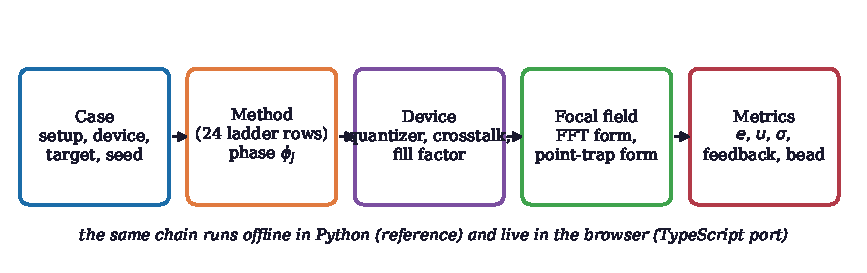
\includegraphics[width=0.95\textwidth]{fig-pipeline.pdf}
\caption{The chain every case runs: a case (optical setup, device, target and seed) is given to a method, which returns a
phase; the device model turns the phase into the field the instrument forms; the metrics score the traps, and the
feedback and particle simulations act on the scored field.}
\label{fig:pipeline}
\end{figure}

\section{The optical model and the device}\label{sec:model}

\subsection{Forward models}

A phase-only SLM of $n_{\mathrm{pix}}\times n_{\mathrm{pix}}$ pixels with pitch $p$ sits in the pupil plane of a lens of
focal length $f$ and wavelength $\lambda$. For a trap $m$ at $(x_m,y_m,z_m)$ with vortex charge $l_m$ the phase delay at
pixel $j$ is
\begin{equation}
\Delta_j^m=\frac{\pi z_m}{\lambda f^2}(x_j^2+y_j^2)+\frac{2\pi}{\lambda f}(x_jx_m+y_jy_m)+l_m\operatorname{atan2}(y_j,x_j),
\end{equation}
and the trap field and intensity are
\begin{equation}
V_m=\frac1{N_{\mathrm{pix}}}\sum_jA_je^{\,i(\phi_j-\Delta_j^m)},\qquad I_m=|V_m|^2,
\end{equation}
with $A_j$ the input beam amplitude normalised so that $\sum_jA_j^2=N_{\mathrm{pix}}=n_{\mathrm{pix}}^2$, following Di Leonardo
et al.~\cite{dileonardo}. $I_m$ is the fraction of the input power in the peak of trap $m$. The second form is the centred,
zero-padded, orthonormal fast Fourier transform (FFT) of the SLM field; at a trap on an FFT bin with $z=0$ and no vortex the two
forms agree exactly, which the test suite checks to $10^{-9}$ rad. One bin of the padded transform spans
$\lambda f/(\mathrm{pad}\,n_{\mathrm{pix}}\,p)$ and the unaliased half-window is $\lambda f/(2p)$; a trap outside it is refused
with the bound (case C11). Depth is handled by the angular spectrum with the band limit of evanescent components removed; the
model is scalar and paraxial, so a high numerical aperture is flagged as outside its validity (case C07).

\subsection{Metrics}

With $I_m$ the trap intensities divided by their target weights, DinHot reports
\begin{equation}
e=\sum_mI_m,\qquad u=1-\frac{\max I-\min I}{\max I+\min I},\qquad \sigma=100\,\frac{\operatorname{std}(I)}{\operatorname{mean}(I)}\ \%,
\end{equation}
the efficiency, the uniformity ($u=1$ is perfect) and the relative standard deviation. Polin et al.~\cite{polin} use the same ratio
without the leading $1-$, a non-uniformity; the two are not mixed. A power budget separates the traps, the zero order, the ghost
traps (everything else on the grid, including folded replicas) and the remainder.

\subsection{The device}

A real SLM quantizes the phase, couples neighbouring pixels, covers only part of each pixel and fluctuates. The device model
applies, in order, wrapping, quantization to $2^b$ levels, a nonlinear response, Gaussian flicker of stated rms and wrapping, and
blurs the upsampled phase with the crosstalk kernel
\begin{equation}
K=\mathcal F^{-1}\Big\{\exp\Big[-\frac{|k_x|^q+|k_y|^q}{\sigma^q}\Big]\Big\},\qquad \sigma=1.24,\ q=1.80,
\end{equation}
the fitted parameters of Schroff et al.~\cite{schroff} on $3\times3$ sub-pixels (error below 2 percent in that work). A square
pixel of fill factor $\mathrm{fill}$ multiplies the focal field by a product of cardinal sines, so the intensity falls to about
$0.4$ at the edge of the unaliased window; this envelope is derived in the engine and tested against a brute-force transform.
The adjoint of the crosstalk operator is closed form (convolution with the reversed kernel and a block sum), which lets
gradient methods differentiate through the device without automatic differentiation. Zernike aberrations follow the Noll
indexing~\cite{noll}. Table~\ref{tab:setups} lists the three optical setups of the cases.

\begin{table}[t]
\centering\footnotesize
\caption{The optical setups of the cases, read from the committed manifests and traces. The device row of C08 is the device the
benchmark also uses for its device cells.}
\label{tab:setups}
\begin{tabular}{@{}l r r r r r r r r@{}}
\toprule
Setup & $\lambda$ (nm) & $f$ (mm) & NA & SLM pixels & pitch ($\mu$m) & pad & bin ($\mu$m) & half field ($\mu$m)\\
\midrule
Atom (C01--C04, C09--C13) & \atomLambda & \atomFocal & \atomNa & $\atomNpix^2$ & \atomPitch & \atomPad & \atomBin & \atomHalf\\
Bead (C05--C07, water) & \beadLambda & \beadFocal & \beadNa & $\beadNpix^2$ & \beadPitch & \beadPad & \beadBin & \beadHalf\\
C08 & \devcLambda & \devcFocal & \devcNa & $\devcNpix^2$ & \devcPitch & \devcPad & \devcBin & \devcHalf\\
C14 & \voluLambda & \voluFocal & \voluNa & $\voluNpix^2$ & \voluPitch & \voluPad & \voluBin & \voluHalf\\
\bottomrule
\end{tabular}

\smallskip
\footnotesize The bead setup is in water of index \beadNimm; C14 is the volume of the released learned model. C08 device: \devcBits-bit phase, crosstalk $\sigma=1.24$, $q=1.80$ on $3\times3$ sub-pixels, fill factor \devcFill, flicker \devcFlicker{} rad.
\end{table}

\section{The three tiers of methods}\label{sec:tiers}

The design document fixes, before any code, a ladder of \nLadder{} rows: \nClassical{} classical methods (the established
methods of the problem), \nSota{} state-of-the-art methods (current solutions, replicated or implemented, never only cited) and
\nBeyond{} proposals beyond the state of the art. Each row has one measurable acceptance criterion and one test. Table~\ref{tab:ladder}
lists them; Table~\ref{tab:acceptance} gives what each test measured on DinHot's own grids, with the seeds stated.

\subsection{Classical tier}

\textbf{Analytic baselines (M01 to M03).} The superposition of prisms and lenses, random superposition (each trap's phase
drawn at random) and the random mask (each pixel assigned to one trap) are the references for the other methods. On the
calibration task of Di Leonardo et al.~\cite{dileonardo} they show the published order: superposition is efficient only by
accident and nearly non-uniform, random superposition gains efficiency at a spread, and the random mask has an efficiency of
about the inverse of the number of traps. \textbf{Gerchberg--Saxton family (M04 to M06).} GS iterates between the SLM and the
trap fields; the generalized adaptive additive form (GAA) adapts the update; weighted GS (GSW)
rescales the target weights by the ratio of the mean to the achieved trap amplitude, $w_m\leftarrow w_m\langle r\rangle/r_m$,
and reaches uniformity close to one~\cite{dileonardo}. \textbf{Direct search (M09)} minimizes the cost
$C=-\langle I\rangle+f\sigma$ pixel by pixel over eight phase levels~\cite{polin}. \textbf{Zernike correction (M14)} recovers
injected aberrations by a sensorless modal search~\cite{noll}. \textbf{Laguerre--Gaussian vortex traps (M15)} wind the
ring phase by $2\pi l$. \textbf{Multi-plane GS (M19)} propagates plane by plane with an amplitude constraint per plane~\cite{whyte}.

\subsection{State-of-the-art tier}

\textbf{Phase-fixed weighted GS (M07)} freezes the focal-plane phase after $N$ iterations so that later iterations adjust only
amplitudes~\cite{kim2019}; the source reports 1500 foci at 91.2 percent modulation efficiency and camera correction to
1.59 percent in three steps against 6.47 percent for conventional weighted GS. DinHot finds that the source default of
$N=12$ stalls on a crowded $50\times30$ array and uses $N=60$ there (Table~\ref{tab:acceptance}). \textbf{MRAF (M08)} frees
a region outside the signal and trades efficiency for accuracy on shaped potentials~\cite{pasienski}. \textbf{Conjugate-gradient
minimization (M10)} uses powered intensity costs and an analytic gradient obtained from two FFTs~\cite{harte}.
\textbf{Wirtinger gradient descent with Adam (M11)} differentiates any forward model through the complex gradient~\cite{chakra}.
\textbf{Closed-loop weighted GS (M12)} corrects trap amplitudes from a camera; DinHot runs it on an emulated camera whose
errors are stated parameters, after Nogrette et al.~\cite{nogrette}; the emulator reproduces the published feedback curves in the browser within the factor set in the design document (Table~\ref{tab:acceptance}) and serves as a validation tool, not as a proposal. \textbf{Device-aware conjugate gradient (M13)} places the
crosstalk kernel in the loop~\cite{schroff}. \textbf{Hungarian assignment and linear phase interpolation (M16)} sorts atoms with a
cost $\sum d^\alpha$, $\alpha>1$, which avoids crossings, and moves them along interpolated holograms~\cite{lee2017,lpi}.
\textbf{An unsupervised convolutional network refined by GS (M17)} follows DeepCGH~\cite{eybposh}. \textbf{Optimal-transport
initialization of MRAF (M18)} seeds the phase from a transport map~\cite{swan,torchylo}.

Of the \benchNProtocol{} engine methods, \nMethodsBaked{} ran in the bake of the cases: \notBakedSentence. The two learned slots answer
with the released graph (M17, on C14) or, with no model released, with their baseline (B3; Section~\ref{sec:learned}).

\begin{longtable}{@{}p{0.07\textwidth} p{0.14\textwidth} p{0.34\textwidth} p{0.40\textwidth}@{}}
\caption{The method ladder of the design document: identifier, tier, method and acceptance criterion.}\label{tab:ladder}\\
\toprule Id & Tier & Method & Acceptance criterion\\\midrule\endfirsthead
\toprule Id & Tier & Method & Acceptance criterion\\\midrule\endhead
M01 & Classical & Superposition of prisms and lenses & \footnotesize on the 10x10 task with a flat beam, efficiency within 0.10 of 0.29 and uniformity below 0.05\\
M02 & Classical & Random superposition & \footnotesize on the 10x10 task with a flat beam, efficiency above M01 and at least 0.65; uniformity below 0.35 (DinHot measured 0.25 at 256 squared against 0.01 at 768 squared in the source; the ordering, not the value, transfers)\\
M03 & Classical & Random mask & \footnotesize efficiency about 1/M; at the source's 768 squared grid, uniformity within the spread of 0.58\\
M04 & Classical & Gerchberg-Saxton, point-trap and FFT forms & \footnotesize the two forms agree to $10^{-9}$ rad; 30 iterations on the 10x10 task with a flat beam reach efficiency at least 0.9 and uniformity near 0.6\\
M05 & Classical & Generalized adaptive additive & \footnotesize uniformity above GS at equal iterations on the 10x10 task\\
M06 & Classical & Weighted GS & \footnotesize efficiency and uniformity at least 0.9 within a median of 15 iterations on the 10x10 task with a flat beam (the source reports about 10); the 3x3x3 lattice above 0.9 and 0.98\\
M07 & State of the art & Phase-fixed weighted GS & \footnotesize fewer iterations than M06 to a relative standard deviation of 0.5 percent on a 50x30 array, with the phase fixed after 60 iterations (DinHot's measured default; at the source's 12 it stalls at 2.9 percent on this grid)\\
M08 & State of the art & MRAF & \footnotesize on disc, ring and bar targets, signal-region error at least five times below GS at the cost of efficiency\\
M09 & Classical & Direct search & \footnotesize uniformity at least 0.98 on the 10x10 task; under 5 percent rms variation on a quasi-periodic set\\
M10 & State of the art & Conjugate-gradient minimization & \footnotesize the analytic gradient matches finite differences; a square lattice below 1 percent error\\
M11 & State of the art & Wirtinger gradient descent with Adam & \footnotesize lower trap-intensity error than M04 at equal iterations on the 10x10 task\\
M12 & State of the art & Closed-loop WGS on an emulated camera & \footnotesize from a 19 percent rms open-loop spread, at most 2.1 percent in 20 iterations at gain 0.7\\
M13 & State of the art & Device-aware CG with pixel crosstalk & \footnotesize on the crosstalk device, lower error than M10 without the model on a large disc\\
M14 & Classical & Zernike correction and sensorless modal recovery & \footnotesize recovers an injected set of Noll modes 4 to 11 within 5 percent of their amplitude\\
M15 & Classical & Laguerre-Gaussian vortex traps & \footnotesize the ring phase winds by 2 pi l with an error under 0.1 rad\\
M16 & State of the art & Hungarian assignment and linear phase interpolation & \footnotesize no crossing moves for alpha 1.5 on a 7x7 to 3x3 sort; a moving trap above 70 percent of its mean intensity\\
M17 & State of the art & Unsupervised CNN hologram refined by GS (DeepCGH-style start) & \footnotesize on held-out targets, the network start followed by GS refinement inside the same wall-clock budget reaches a higher accuracy than GS alone (measured alone, the network matches GS at equal time: median ratio 0.998)\\
M18 & State of the art & Optimal-transport initialized MRAF & \footnotesize lower error than MRAF from a random start on the shaped targets\\
M19 & Classical & Multi-plane GS & \footnotesize on a three-plane target, every plane mean within 25 percent of the overall mean (volumetric 3D GS of Whyte and Courtial)\\
BS-1 & Beyond & Device-aware weighted GS (engine id B1) & \footnotesize on the crosstalk device, relative standard deviation at least two times below M07, efficiency at most 10 percent lower\\
BS-2 & Beyond & Flicker-bounded phase-continuous sequence (engine id B2) & \footnotesize minimum transient intensity of a moving trap at least 0.9 of its mean, against LPI\\
BS-3 & Beyond & Learned warm start for phase-fixed WGS (refuted) (engine id B3) & \footnotesize measured negative: on held-out geometries the network start needs a median 8 iterations to 1 percent against 14 from a random start (1.75 times, below the 2 times claimed), and a control with the same early phase fix and no network gains as much; the model is not released and the claim BS-3 is reported as refuted\\
BS-4 & Beyond & Aberration-robust hologram (engine id B4) & \footnotesize over a 200-sample ensemble of residual aberrations, the 95th percentile of the relative standard deviation at least 1.25 times below M07, efficiency at most 10 percent lower; robustness to pointing errors is measured and reported, not claimed (limited by the spot width: 1.02 times)\\
BS-5 & Beyond & Efficiency-uniformity Pareto front (engine id B5) & \footnotesize hypervolume at least that of the M04, M05, M09 and M06 points on the 10x10 task\\
\bottomrule\end{longtable}

\begin{longtable}{@{}p{0.07\textwidth} p{0.74\textwidth} p{0.13\textwidth}@{}}
\caption{Measured acceptance of the methods on DinHot's own grids (unit tests; seeds as stated). Intervals are [min, max].}\label{tab:acceptance}\\
\toprule Id & Measured & Seeds\\\midrule\endfirsthead
\toprule Id & Measured & Seeds\\\midrule\endhead
M01 & \footnotesize efficiency 0.281, uniformity 0.0003 (deterministic) & \footnotesize 1\\
M02 & \footnotesize efficiency 0.750 [0.738, 0.752], uniformity 0.252 [0.106, 0.272] & \footnotesize 6\\
M03 & \footnotesize 256 squared: efficiency 0.010, uniformity 0.057 [0.031, 0.072]; 768 squared: efficiency 0.008, uniformity 0.566 [0.543, 0.590] & \footnotesize 5 and 2\\
M04 & \footnotesize flat beam: efficiency 0.939 [0.933, 0.939], uniformity 0.604 [0.557, 0.626]; Gaussian beam: efficiency 0.815 & \footnotesize 5\\
M05 & \footnotesize uniformity 0.688 [0.638, 0.709] against 0.615 [0.550, 0.637] for GS at equal iterations & \footnotesize 5\\
M06 & \footnotesize efficiency and uniformity both at 0.9 after 10 to 13 iterations (flat and Gaussian beams); 3 x 3 x 3 lattice reaches 0.9 and 0.98 & \footnotesize 3\\
M07 & \footnotesize 50 x 30 array to 0.5 percent in 63 and 64 iterations against 121 and 147 for M06 (phase fixed after 60); with the source value of 12 it stalls at 2.88 percent & \footnotesize 2\\
M08 & \footnotesize signal-region error 14.5 (disc), 7.9 (ring) and 12.1 (bar) times below GS; efficiency 0.18 against 0.97 to 0.99 & \footnotesize 3\\
M09 & \footnotesize uniformity 0.9994 and 0.9992 (efficiency 0.66 and 0.65); 119 quasi-periodic traps at 0.023 percent rms & \footnotesize 2 and 1\\
M10 & \footnotesize analytic gradient within 1.8e-7 of finite differences; square lattice error 0.55 and 0.51 percent & \footnotesize 2\\
M11 & \footnotesize relative standard deviation 2.54, 2.46 and 2.26 percent against 17.79, 17.98 and 18.82 for GS at 30 iterations & \footnotesize 3\\
M12 & \footnotesize emulated camera loop: open-loop 20.9 and 20.1 percent to 1.47 and 1.08 percent in 20 iterations; 24.3 and 23.4 percent to 0.77 and 0.53 percent in three phase-fixed steps & \footnotesize 2\\
M13 & \footnotesize error 0.241 (efficiency 0.535) against 1.38 (0.507) for M10 without the device model, large disc on the crosstalk device & \footnotesize 1\\
M14 & \footnotesize worst per-mode relative error 0.002 [0.001, 0.002] over Noll modes 4 to 11 & \footnotesize 3\\
M15 & \footnotesize ring phase winds by 2 pi l with a maximum error of 0.033 rad [0.028, 0.060] (isolated vortex) & \footnotesize 3\\
M16 & \footnotesize 0 path crossings in 60 loadings; moving traps keep 0.870 [0.748, 0.963] of their mean intensity & \footnotesize 60 loadings\\
M17 & \footnotesize three-plane network refined by M19: median accuracy ratio 1.140 [1.102, 1.160] on 162 held-out volumes & \footnotesize 162 volumes\\
M18 & \footnotesize signal-region error 0.0204 (disc), 0.0179 (ring) and 0.0221 (line) against 0.250, 0.192 and 0.250 for MRAF from a random start & \footnotesize 1\\
M19 & \footnotesize plane means over overall mean 0.938, 0.987, 1.075 and 0.926, 1.034, 1.039 on three planes & \footnotesize 2\\
BS-4 & \footnotesize 95th percentile of the relative standard deviation 4.045 against 6.268 for M07 (1.55 times) over a 200-sample aberration ensemble; efficiency 0.7031 against 0.7169; pointing errors 1.02 times & \footnotesize 1\\
BS-5 & \footnotesize hypervolume 0.8201 against 0.8033 for the union of the GS-family points; one front point dominates M04 and M05 & \footnotesize 1\\
\bottomrule\end{longtable}


\section{The cases}\label{sec:cases}

A case is an optical setup, a device, a target (a list of traps or a shaped potential), an aberration, a method set, a seed and,
for dynamic cases, a particle and a rearrangement. There are \nCases{} cases in four categories (Table~\ref{tab:cases}):
arrays (a $3\times3$ grid, a $10\times10$ grid with camera feedback, a $32\times32$ array of \maxTraps{} traps, the calibration
task and a disordered array of \nDisordered{} traps on integer FFT bins at least five bins apart), shaped and three-dimensional
targets (a disc potential with the crosstalk model, a three-plane array with vortices, a vortex ring with a line, and a three-plane volume
at the geometry of the released learned model), device and
optics (high numerical aperture, a device-limited array, an aberrated array with and without correction) and dynamics and
controls (an atom-rearrangement sequence and a trap outside the field, which is refused and never computed). Every case states
numeric expected ranges for its metrics, measured on three seeds, and the bake fails outside them. All cases are synthetic:
the parameters are stated and no measured sample is used. The baked cases span \minTraps{} to \maxTraps{} traps.

\begin{table}[t]\centering\footnotesize
\caption{The thirteen cases: category, optical setup, target and the methods that ran in the bake. C11 is refused by the input contract and never computed.}\label{tab:cases}
\begin{tabular}{@{}l l l l r l@{}}\toprule Case & Category & Setup & Target & Methods & Reference\\\midrule
C01 & Arrays & 850 nm, NA 0.5 & 9 traps & 13 & M06\\
C02 & Arrays & 850 nm, NA 0.5 & 100 traps & 13 & M07\\
C03 & Arrays & 850 nm, NA 0.5 & 1024 traps & 6 & M07\\
C04 & Shaped and 3D & 850 nm, NA 0.5 & disc potential, 8-bit & 6 & M13\\
C05 & Shaped and 3D & 1064 nm, NA 1.2 & 51 traps & 10 & M09\\
C06 & Shaped and 3D & 1064 nm, NA 1.2 & 25 traps & 8 & M07\\
C07 & Device and optics & 1064 nm, NA 1.2 & 25 traps & 12 & M07\\
C08 & Device and optics & 850 nm, NA 0.5 & 64 traps, 4-bit, fill 0.85 & 7 & B1\\
C09 & Device and optics & 850 nm, NA 0.5 & 16 traps, aberrated & 6 & M14\\
C10 & Dynamics and controls & 850 nm, NA 0.5 & 100 traps & 4 & M16\\
C11 & Dynamics and controls & & one trap at 200 $\mu$m, outside the field & 0 & refused\\
C12 & Arrays & 850 nm, NA 0.5 & 100 traps & 7 & M06\\
C13 & Arrays & 850 nm, NA 0.5 & 819 traps & 6 & M07\\
\bottomrule\end{tabular}\end{table}


\begin{figure}[t]
\centering
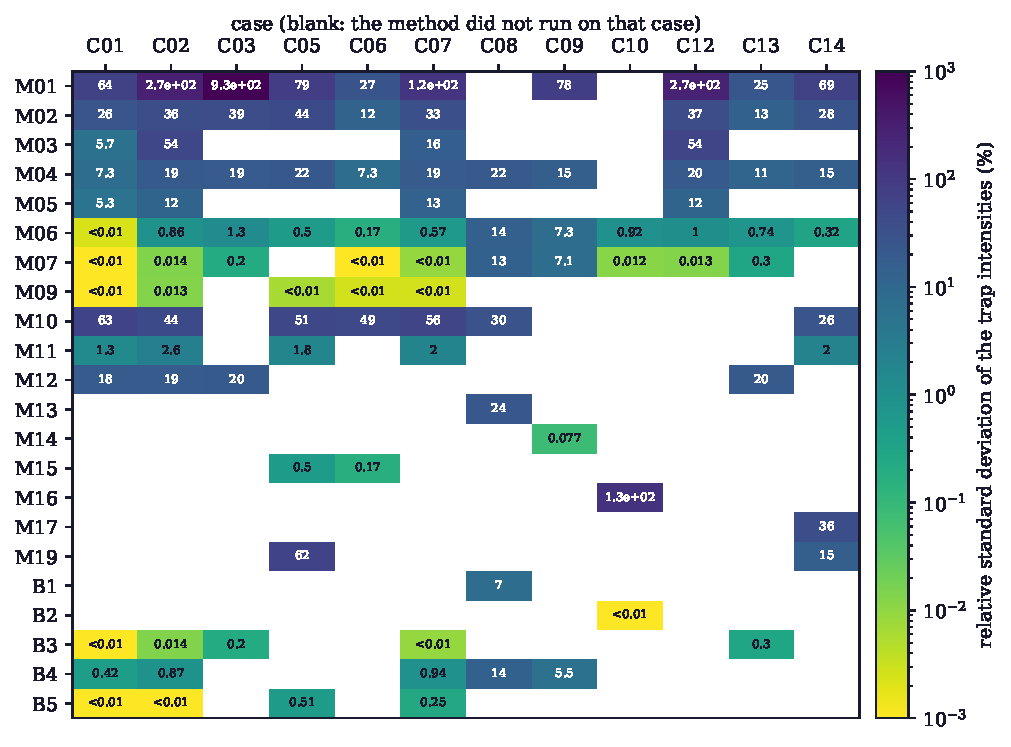
\includegraphics[width=0.92\textwidth]{fig-cases.pdf}
\caption{Relative standard deviation of the trap intensities, every method on every point-trap case of the bake (the
shaped-potential case C04 is scored on its signal region and is omitted). Each cell is one method run at the case budget.
Plain Gerchberg--Saxton (M04) leaves the largest spreads; the weighted and phase-fixed forms (M06, M07), the direct
search (M09), the Pareto front (B5) and the device-aware methods remove most of it where they apply.}
\label{fig:cases}
\end{figure}

\section{Protocols and results}\label{sec:results}

\subsection{Baked cases}

Each case is computed offline with every method valid for it (the seed is stated in each manifest), checked against its expected
ranges, and committed as a manifest and a trace of at most \liveTraceKiB{} KiB. Table~\ref{tab:calibration} compares the
calibration case with the published rows of Di Leonardo et al.: the ordering of the six baselines and the weighted-GS
uniformity are reproduced; the efficiencies of the GS family are lower than published because the engine's Gaussian input beam
caps the efficiency, whereas the source uses a flat beam (the flat-beam test of M04 gives \accFourFlatEff{} efficiency and \accFourFlatUni{}
uniformity; Table~\ref{tab:acceptance}). The DinHot uniformity of random superposition and of the random mask differ from the
published values on the engine's smaller grid, as the acceptance test of those methods states: the order, not the value, transfers.

\begin{table}[t]\centering\footnotesize
\caption{Calibration case C12 (10 $\times$ 10 traps at eight Fourier units): efficiency $e$ and uniformity $u$ of the analytic and Gerchberg--Saxton baselines as baked, against the values published by Di~Leonardo et al.\ for the same task.}\label{tab:calibration}
\begin{tabular}{@{}l r r r r r@{}}\toprule Method & $e$ (baked) & $u$ (baked) & $\sigma$ (\%) & $e$ (published) & $u$ (published)\\\midrule
M01 & 0.328 & 0.000 & 268.79 & 0.29 & 0.01\\
M02 & 0.749 & 0.199 & 37.40 & 0.69 & 0.01\\
M03 & 0.010 & 0.077 & 54.25 & 0.01 & 0.58\\
M04 & 0.817 & 0.506 & 19.97 & 0.94 & 0.60\\
M05 & 0.818 & 0.738 & 11.81 & 0.93 & 0.79\\
M06 & 0.805 & 0.970 & 1.02 & 0.93 & 0.99\\
M07 & 0.797 & 1.000 & 0.01 & n/a & n/a\\
\bottomrule\end{tabular}\end{table}

\begin{table}[t]\centering\footnotesize
\caption{Baked results per case at the case budget: the method with the lowest relative standard deviation among those with at least half the best efficiency, and the phase-fixed WGS (M07) and plain GS (M04) rows where they ran. $e$ efficiency, $\sigma$ relative standard deviation of the trap intensities (\%).}\label{tab:results}
\begin{tabular}{@{}l l r r r r r@{}}\toprule Case & Best & $e$ & $\sigma$ & M07 $\sigma$ & M07 $e$ & M04 $\sigma$\\\midrule
C01 & B5 & 0.817 & $<$0.01 & $<$0.01 & 0.817 & 7.3\\
C02 & B5 & 0.798 & $<$0.01 & 0.01 & 0.798 & 19.5\\
C03 & M07 & 0.794 & 0.20 & 0.20 & 0.794 & 18.7\\
C04 & shaped potential & n/a & n/a & n/a & n/a & n/a\\
C05 & M09 & 0.699 & 0.01 & n/a & n/a & 22.4\\
C06 & M07 & 0.704 & $<$0.01 & $<$0.01 & 0.704 & 7.3\\
C07 & M09 & 0.638 & $<$0.01 & 0.01 & 0.791 & 18.7\\
C08 & B1 & 0.652 & 7.05 & 13.42 & 0.675 & 21.6\\
C09 & M14 & 0.805 & 0.08 & 7.09 & 0.453 & 15.0\\
C10 & B2 & 0.798 & $<$0.01 & 0.01 & 0.797 & n/a\\
C12 & M07 & 0.797 & 0.01 & 0.01 & 0.797 & 20.0\\
C13 & M07 & 0.723 & 0.30 & 0.30 & 0.723 & 11.2\\
C14 & M06 & 0.785 & 0.32 & n/a & n/a & 15.3\\
\bottomrule\end{tabular}\end{table}


Table~\ref{tab:results} summarizes the baked cases. Where both ran, phase-fixed weighted GS (M07) leaves a median relative
standard deviation of \medSigmaMseven{} percent against \medSigmaMfour{} percent for plain GS (M04) over \nBothFourSeven{} cases,
at efficiencies between \minEffMseven{} and \maxEffMseven. On the device-limited case C08 phase-fixed weighted GS (M07), which ignores the
device, keeps a spread of \bakeCeightMsevenSigma{} percent, and the device-aware weighted GS (B1) lowers it to \bakeCeightBOneSigma{} percent, a factor of
\bakeCeightRatio{}, on that small grid (the larger task of Section~\ref{sec:beyond} gives a larger factor; both are reported in the companion
manuscript). On the aberrated case C09, correction of the Zernike modes (M14) restores efficiency and uniformity that
the uncorrected methods lose.

\begin{figure}[t]
\centering
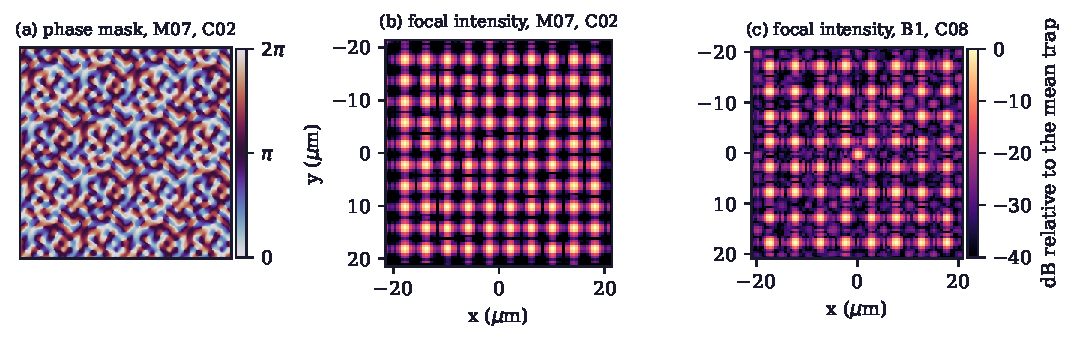
\includegraphics[width=\textwidth]{fig-maps.pdf}
\caption{(a) Phase mask of the reference method on C02. (b) Its focal intensity, in dB relative to the mean trap, on the ideal device:
a regular lattice. (c) The focal intensity of the device-aware weighted GS on C08, scored on the device with 4-bit
phase, crosstalk and a fill factor of \devcFill: the traps are visible and not equal.}
\label{fig:maps}
\end{figure}

\subsection{Feedback and particles}

The emulated camera loop reduces the spread as in the published curves. In the baked traces the relative standard deviation
falls from \fbCOneStart{} to \fbCOneEnd{} percent in \fbCOneSteps{} steps on C01, from \fbCTwoStart{} to \fbCTwoEnd{} percent in \fbCTwoSteps{}
steps on the $10\times10$ grid C02, from \fbCThreeStart{} to \fbCThreeEnd{} percent in \fbCThreeSteps{} steps on the large array C03, and from
\fbCThirteenStart{} to \fbCThirteenEnd{} percent in \fbCThirteenSteps{} steps on the disordered array C13 (Fig.~\ref{fig:feedback}). The published
closed-loop result of Nogrette et al.~\cite{nogrette} is a trap-depth spread of 19 percent rms reduced to 1.4 percent in 20
iterations; the unit test of M12 reproduces it within the factor set in the design document (Table~\ref{tab:acceptance}).
The particle simulations act on the computed traps: C01 carries a bead in the central trap (stiffness \beadKappa{} pN/$\mu$m and a
corner frequency of \beadFc{} Hz in the trace) and C03 an atom (a corner frequency of \atomFc{} Hz and a radial trap frequency of
\atomOmega{} Hz in the trace); the trap depth follows the intensity~\cite{grimm}, and the bead's spectrum is a Lorentzian
whose corner frequency is the stiffness over $2\pi\gamma$~\cite{tolic}, which the particle oracle checks.

\begin{figure}[t]
\centering
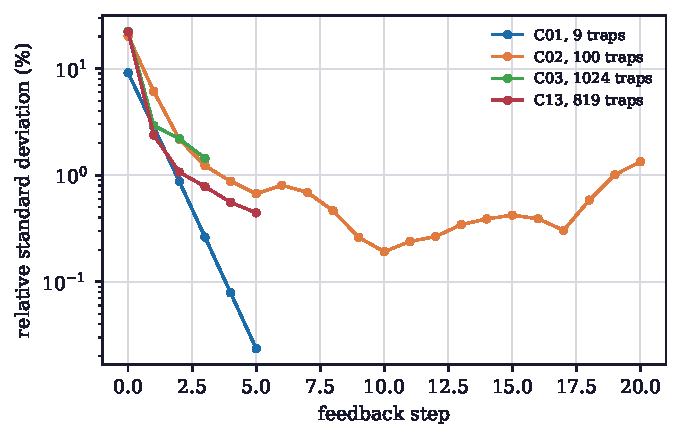
\includegraphics[width=0.62\textwidth]{fig-feedback.pdf}
\caption{Emulated camera feedback: relative standard deviation of the trap intensities against the feedback step, on four cases (baked traces).}
\label{fig:feedback}
\end{figure}

\subsection{The benchmark protocol}

The benchmark compares the tiers on one protocol. Its geometries are (\benchGeometries{}) a $10\times10$ square, a ring of 36 traps, 100 random
traps, a quasi-periodic set of 119, a $5\times5\times3$ lattice, a large array ($32\times32$ and the disordered 819 set) and shaped fields;
the grids are \benchGrids{} pixels, the iteration budgets are \benchIters{} and the time budgets are \benchTimes{} s (the last is
the converged row). Every cell runs on \benchSeeds{} seeds and reports the median and the inter-quartile range of efficiency,
uniformity, relative standard deviation, time and iterations, on the ideal device and on the C08 device (every hologram scored
against its device). The Pareto fronts are stored with the cells.

The committed results file holds \benchRows{} rows of the \benchNMeasured{} engine methods; \benchSkipped{} method--geometry cells are
recorded as skipped with the reason the file states (a method that does not accept the target, such as a two-dimensional method on a
three-dimensional lattice, or one that refuses the geometry). A cell runs between \benchSeedsMin{} and \benchSeedsMax{} seeds, the bound the protocol
puts on the wall clock of a group. Table~\ref{tab:benchmark} names, per geometry and device, the method of each tier with the lowest median spread at
100 iterations among those that reach at least half of the cell's best efficiency, and the best method at a time budget of 1~s;
Table~\ref{tab:benchmethods} gives the medians of every method over the \benchNPoint{} point-trap geometries, and Fig.~\ref{fig:bench} every cell.

On the ideal device the best method of a geometry is classical on \benchWinsIdealClassical, state of the art on \benchWinsIdealSota{} and beyond on
\benchWinsIdealBeyond{} of the \benchGeoIdeal{} geometries; on the C08 device the counts are \benchWinsDeviceClassical, \benchWinsDeviceSota{} and
\benchWinsDeviceBeyond{} of \benchGeoDevice{} (the multi-plane geometry has no device rows). Over the point-trap geometries the lowest median spread
on the ideal device is that of \benchBestIdeal{} (\benchBestIdealSigma{} percent at a median efficiency of \benchBestIdealEff), and on the C08 device
that of \benchBestDevice{} (\benchBestDeviceSigma{} percent at \benchBestDeviceEff). The medians of the \benchSpreadIdealN{} methods that keep at least
half of the best efficiency span \benchSpreadIdealLow{} to \benchSpreadIdealHigh{} percent on the ideal device and \benchSpreadDeviceLow{} to
\benchSpreadDeviceHigh{} percent (\benchSpreadDeviceN{} methods) on the C08 device, where every method runs with its default parameters and only the
device-aware ones model the device. The times are wall-clock seconds of the machine that ran the benchmark, under shared load.

\begin{table}[t]\centering\footnotesize
\caption{Benchmark cells measured so far in the committed results file (budget of 100 iterations, medians over the seeds). A cell absent from the file is not yet measured.}\label{tab:benchmark}
\begin{tabular}{@{}l l l r r r@{}}\toprule Method & Geometry & Device & Seeds & $e$ & $\sigma$ (\%)\\\midrule
M01 & G1 & device & 20 & 0.193 & 264.60\\
M01 & G1 & ideal & 20 & 0.328 & 268.79\\
M01 & G2 & device & 20 & 0.339 & 3.69\\
M01 & G2 & ideal & 20 & 0.568 & 2.12\\
M01 & G3 & device & 20 & 0.512 & 13.22\\
M01 & G3 & ideal & 20 & 0.672 & 7.84\\
M01 & G4 & device & 20 & 0.313 & 160.55\\
M01 & G4 & ideal & 20 & 0.426 & 106.34\\
M01 & G5 & ideal & 20 & 0.328 & 143.53\\
\bottomrule\end{tabular}\end{table}

\begin{table}[p]\centering\footnotesize
\caption{Benchmark, per method: medians over the point-trap geometries the method ran on (of 6) at 100 iterations with the default parameters, on the ideal device and on the C08 device. $\sigma$ relative standard deviation (\%), $e$ efficiency, time wall-clock seconds under shared load.}\label{tab:benchmethods}
\begin{tabular}{@{}l l r r r r r r@{}}\toprule Id & Tier & Geometries & $\sigma$ ideal & $e$ ideal & time (s) & $\sigma$ C08 & $e$ C08\\\midrule
M01 & Classical & 5 & 106 & 0.426 & 0.027 & 87 & 0.326\\
\bottomrule\end{tabular}\end{table}


\begin{figure}[t]
\centering
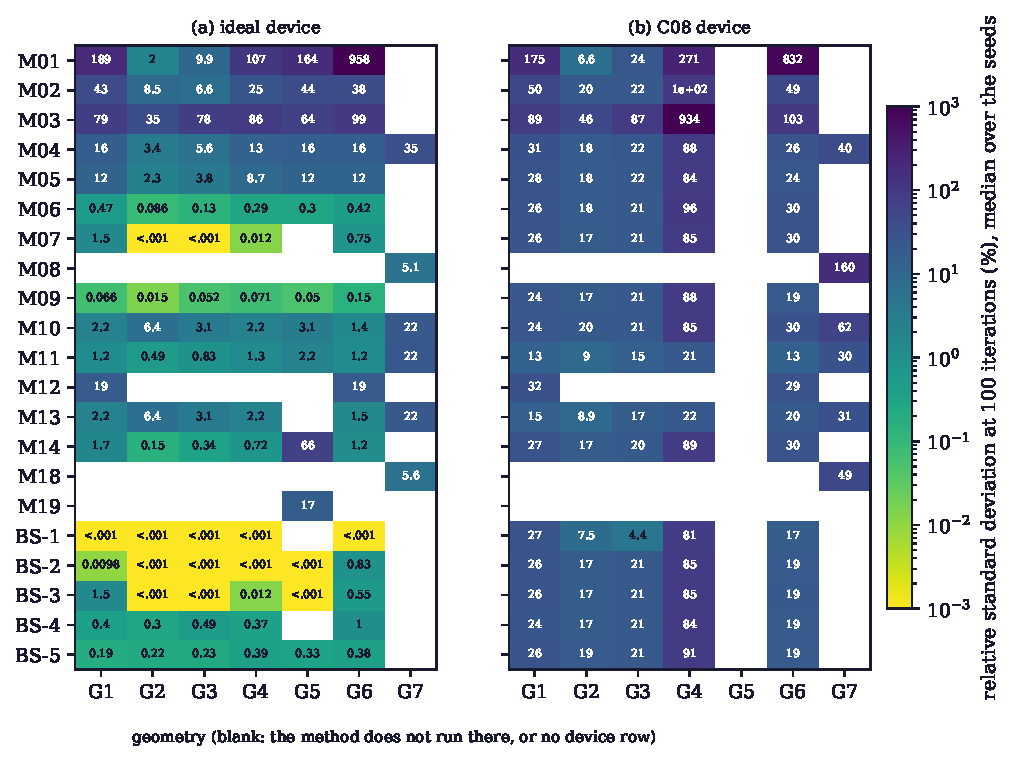
\includegraphics[width=\textwidth]{fig-bench.pdf}
\caption{Benchmark: median relative standard deviation at 100 iterations with the default parameters, every method on every geometry, on the ideal
device (a) and on the C08 device (b). Blank: the method does not accept the geometry or refuses it, or the geometry has no device row.}
\label{fig:bench}
\end{figure}

\section{The learned models}\label{sec:learned}

Two networks were trained offline with PyTorch, exported to ONNX with a list of operators the browser runtime supports, and
evaluated on held-out sets written before the final training with other seeds. A model is released only if it meets its
criterion; otherwise the baseline answers.

\textbf{cgh-net (M17).} A U-Net maps three plane amplitudes, at $-8$, $0$ and $+8$ SLM-limited Rayleigh ranges, to one phase for the
$128\times128$ SLM, in the setting of DeepCGH~\cite{eybposh}. It is trained without labels through the differentiable FFT model,
with the loss $1-\mathrm{AC}$ over the planes, $\mathrm{AC}=2\sum TI/(\sum T^2+\sum I^2)$ on unit-sum plane intensities, for \cghSteps{}
steps. The exported graph is \cghBytes{} MB. The baseline is volumetric three-dimensional GS (M19) on the same traps with a wall-clock budget
of \cghBudgetS{} s, the median time of M19 at 30 iterations. On \cghN{} held-out volumes the network answers in about \cghNetMs{} ms
with a median accuracy ratio of \cghMed{} (quartiles \cghQOne{} and \cghQThree), above the baseline on \cghShareAbove{} percent of the
volumes; the median accuracy is \cghAcHybrid{} against \cghAcMnine{}. By kind the ratio is \cghLatticeRatio{} (lattices), \cghRandomRatio{} (random),
\cghMixedRatio{} (mixed), \cghRingRatio{} (rings), \cghGfiveRatio{} (the $5\times5\times3$ benchmark lattice) and \cghPlaneRatio{} (the three-plane layout).
The ONNX graph agrees with PyTorch on the reconstructed plane intensities to $\cghParity$ (relative to the maximum). The accuracy measure scores full plane
images, ghosts and blur included, which is what the network optimises; M19 optimises trap uniformity, so the ratio is a statement about this measure.
The two-dimensional counterpart, a single-plane network followed by GS refinement, ties: on \cghTwoDN{} held-out targets the ratio at equal
wall-clock is \cghTwoDMed{}, below the criterion, and that model is not released.

\textbf{warmstart-model (BS-3).} A permutation-equivariant set network predicts initial trap phases for phase-fixed WGS. On \wsN{} held-out
geometries it needs a median of \wsModelIt{} iterations to reach 1 percent against \wsRandomIt{} from a random start (a factor of \wsRatio, below the
factor of two set as the criterion), but only with the early phase freeze (after \wsNfixModel{} iterations, against \wsNfixRandom{} for the random arm). A control with
no network, a random start and the same early freeze, needs a median of \wsControlIt{} iterations on the control subset, and \wsControlNever{} percent of its
geometries never reach 1 percent (\wsModelNever{} percent with the network); the final efficiency differs by \wsEffDiff{} percent between the arms. The gain comes from the
freeze, not from the network, so the proposal is refuted and the model is not released (Fig.~\ref{fig:learned}).

\begin{figure}[t]
\centering
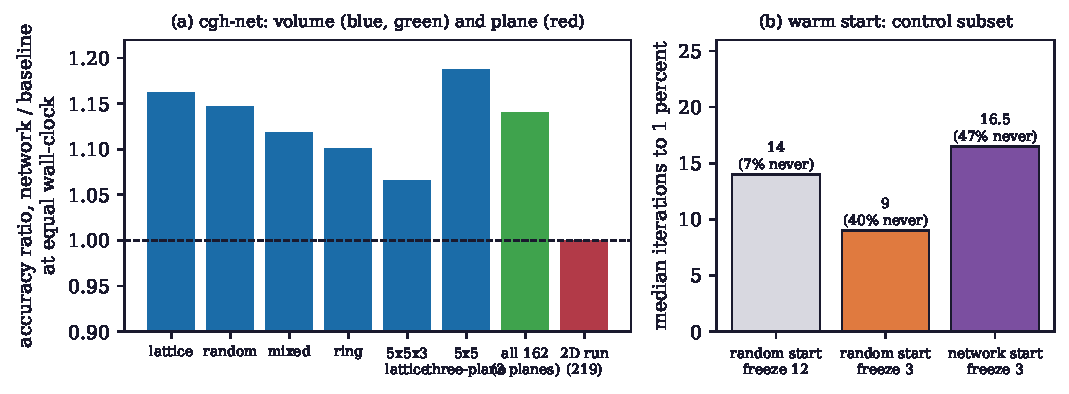
\includegraphics[width=\textwidth]{fig-learned.pdf}
\caption{(a) The cgh-net accuracy ratio over its baseline at equal wall-clock, by target kind on the held-out volumes (G5: the $5\times5\times3$ lattice;
3-plane: the $5\times5$ three-plane layout), for the volume network (blue, green) and the two-dimensional single-plane network (red); the dashed line is the baseline.
(b) The warm-start control: median iterations to 1 percent for a random start with the original and the early freeze and for the network start with the early freeze.}
\label{fig:learned}
\end{figure}

\section{Proposals beyond the published state of the art}\label{sec:beyond}

Each proposal is DinHot's own, grounded in a stated gap, measured against the strongest baseline and reported whether or not it
succeeds.

\textbf{BS-1, device-aware weighted GS.} The weights of weighted GS are kept and the phase update is replaced by conjugate-gradient steps through
the crosstalk kernel and the quantizer. The gap is that the crosstalk model has only been used with conjugate gradient on shaped potentials~\cite{schroff},
or inside a weighted GS that replaces amplitudes only~\cite{persson}. On the crosstalk device, the relative standard deviation is lower than
that of phase-fixed WGS by the factor reported in the companion manuscript; on the small C08 grid the baked factor is \bakeCeightRatio{} at an
efficiency ratio of \bakeCeightEffRatio. \textbf{BS-2, flicker-bounded phase-continuous sequences.} Each intermediate hologram of a moving-trap
sequence is optimized with the trap phases locked to a smooth trajectory; the gap is that linear phase interpolation does not
optimize its intermediate frames~\cite{lpi}. The moving traps keep a higher minimum intensity than under linear phase
interpolation, as quantified in the companion manuscript. \textbf{BS-3, learned warm start:} refuted (Section~\ref{sec:learned}).
\textbf{BS-4, aberration-robust hologram:} the expected cost over residual aberrations is minimized; over a 200-sample ensemble of residual Noll modes 4 to 11
the 95th percentile of the relative standard deviation is \accBFourRatio{} times below that of M07 on the seed of its test, with an efficiency \accBFourEffDrop{}
percent lower (Table~\ref{tab:acceptance}); robustness to pointing errors does not follow (\accBFourPointing{} times), because the spot width bounds
it, and is reported as a negative result. The gap is that corrections are
global or per site, never robust~\cite{machu}. \textbf{BS-5, efficiency--uniformity Pareto front} by continuation of a weighted cost: the front's hypervolume (\accBFiveHv) exceeds
that of the points of the GS family and direct search (\accBFiveHvBase), and \accBFiveDomFour{} front points dominate M04 and \accBFiveDomFive{} dominate M05
(Table~\ref{tab:acceptance}), where published methods report single trade-off points~\cite{dileonardo}.

\section{The live engine and the product}\label{sec:live}

The site is static; every computation runs in the browser or was baked offline and is replayed. The live engine is a TypeScript port of the forward
models, the device model and the live methods, running in a Web Worker so the interface does not block, with the FFT in Float64 (fft.js). An optional WebGPU backend
runs the FFT-form iterations on the GPU and falls back to the CPU path when the browser offers none; an agreement check inside every GPU run compares the trap fields
with the CPU result. At the live grid ($256^2$ padded to $512^2$) a weighted GS iteration measured about \liveIterMs{} ms, so a 30-iteration run fits the lane budget of
\liveBudgetMs{} ms. The Python engine writes \liveFixtures{} reference documents and \liveTests{} parity tests compare the TypeScript engine with them, each quantity within
the tolerance its document states (at most $\liveTol$ absolute). On \liveAdapter{}, 30 iterations of M07 took \liveGpuS{} s with the GPU
backend against \liveCpuS{} s on the CPU path in the same browser. The methods that are baked and replayed are labelled as such in the interface. Of the \nContracts{} data
contracts of the build, \nContractsAvailable{} are fully available, and the build declares the state of the others: \readinessOthers. The refused record is the case outside the field, and the
benchmark counts its skipped cells as not run; the dormant API serves GET requests and answers 503 with the declared state.

\section{Limits}\label{sec:limits}

DinHot computes and evaluates holograms in simulation: it does not drive an SLM or a camera, and its camera-in-the-loop method runs on an emulated
camera whose errors are stated parameters. Device and set-up parameters come from published experiments, so absolute numbers belong to the stated model and not to a measured instrument.
The engine is scalar (Fraunhofer and angular spectrum); the high-numerical-aperture case carries a validity flag and the vectorial lane is not built. The fill-factor, 4-bit and flicker effects of the
device have no published source in this build and are computed only. The crosstalk kernel's frequency unit is carried over from the engine and is not verified against the source. The transient-intensity model of BS-2 is
the engine's own (Section~\ref{sec:beyond} and the companion manuscript) and the linear-phase-interpolation baseline is DinHot's implementation of a published description, not the authors' code. The
unit measurements of Table~\ref{tab:acceptance} use between one and six seeds; the benchmark repeats the methods on its geometries with \benchSeedsMin{} to \benchSeedsMax{} seeds per cell. The cgh-net advantage is on a plane-image accuracy measure over generated volumes and
the benchmark's volumetric layouts, not on a hardware experiment. The learned warm start is refuted and the two-dimensional network ties with GS. The executive figures of the introduction are taken from the cited publications and not re-measured.

\section*{Data and code availability}

The source code, the baked artifacts (manifests, traces, benchmark results, model cards, the ONNX graph and its held-out metrics) and the scripts that regenerate every table and figure of this report from them are in the repository
\url{https://github.com/fsantibanezleal/CEFOP_DinHot} (Apache-2.0), under \texttt{manuscripts/holographic-trap-studio/}; the studio runs at \url{https://dinhot.fasl-work.com}.
Unit measurements quoted in Table~\ref{tab:acceptance} are produced by the tests named in Table~\ref{tab:ladder}.

\begin{thebibliography}{99}\small\raggedright
\bibitem{manetsch} Manetsch \emph{et al.}, ``A tweezer array with 6100 highly coherent atomic qubits,'' \emph{Nature} 647, 60--67, 2025. arXiv:2403.12021.
\bibitem{dileonardo} Di Leonardo, Ianni and Ruocco, ``Computer generation of optimal holograms for optical trap arrays,'' \emph{Opt. Express} 15, 1913, 2007. doi:10.1364/OE.15.001913.
\bibitem{kim2019} Kim, Kim, Lee and Ahn, ``Large-scale uniform optical focus array generation with a phase spatial light modulator,'' \emph{Opt. Lett.} 44, 3178, 2019. doi:10.1364/OL.44.003178.
\bibitem{pasienski} Pasienski and DeMarco, ``A high-accuracy algorithm for designing arbitrary holographic atom traps,'' \emph{Opt. Express} 16, 2176, 2008. doi:10.1364/OE.16.002176.
\bibitem{polin} Polin \emph{et al.}, ``Optimized holographic optical traps,'' \emph{Opt. Express} 13, 5831, 2005. doi:10.1364/OPEX.13.005831.
\bibitem{harte} Harte \emph{et al.}, ``A conjugate gradient minimisation approach to generating holographic traps for ultracold atoms,'' \emph{Opt. Express} 22, 26548, 2014. doi:10.1364/OE.22.026548.
\bibitem{chakra} Chakravarthula \emph{et al.}, ``Wirtinger holography for near-eye displays,'' \emph{ACM Trans. Graph.} (SIGGRAPH Asia), 2019. doi:10.1145/3355089.3356539.
\bibitem{nogrette} Nogrette \emph{et al.}, ``Single-atom trapping in holographic 2D arrays of microtraps with arbitrary geometries,'' arXiv:1402.5329, 2014.
\bibitem{schroff} Schroff, La Rooij, Haller and Kuhr, ``Accurate holographic light potentials using pixel crosstalk modelling,'' \emph{Sci. Rep.}, 2023. doi:10.1038/s41598-023-30296-6.
\bibitem{noll} Noll, ``Zernike polynomials and atmospheric turbulence,'' \emph{J. Opt. Soc. Am.} 66, 207, 1976. doi:10.1364/JOSA.66.000207.
\bibitem{whyte} Whyte and Courtial, ``Experimental demonstration of holographic three-dimensional light shaping using a Gerchberg--Saxton algorithm,'' \emph{New J. Phys.} 7, 117, 2005. doi:10.1088/1367-2630/7/1/117.
\bibitem{lee2017} Lee, Kim and Ahn, ``Defect-free atomic array formation using the Hungarian matching algorithm,'' \emph{Phys. Rev. A} 95, 053424, 2017. doi:10.1103/PhysRevA.95.053424.
\bibitem{lpi} ``Parallel assembly of neutral atom arrays with an SLM using linear phase interpolation,'' arXiv:2501.01391.
\bibitem{eybposh} Eybposh \emph{et al.}, ``DeepCGH: 3D computer-generated holography using deep learning,'' \emph{Opt. Express} 28, 26636, 2020. doi:10.1364/OE.399624.
\bibitem{swan} Swan \emph{et al.}, ``High-fidelity holographic beam shaping with optimal transport and phase diversity,'' arXiv:2408.17025.
\bibitem{torchylo} Torchylo \emph{et al.}, ``A fast, large-scale optimal transport algorithm for holographic beam shaping,'' arXiv:2512.19072.
\bibitem{persson} Persson, Engstr\"om and Goks\"or, ``Reducing the effect of pixel crosstalk in phase only spatial light modulators,'' \emph{Opt. Express} 20, 22334, 2012.
\bibitem{machu} Machu \emph{et al.}, ``Full-field-of-view aberration correction for large arrays of focused beams,'' arXiv:2512.15967.
\bibitem{grimm} Grimm, Weidem\"uller and Ovchinnikov, optical dipole traps for neutral atoms, arXiv:physics/9902072, 2000.
\bibitem{tolic} Tol\'i\'c-N{\o}rrelykke \emph{et al.}, stiffness calibration of optical traps from the power spectrum, arXiv:physics/0603037, 2006.
\end{thebibliography}

\end{document}
